\documentclass[10pt,xcolor=table]{beamer}

\usepackage{graphicx}
\usepackage{caption}
\usepackage{subcaption}
 
% \usepackage[utf8]{inputenc}
% \usepackage[T1]{fontenc}
\usepackage[table]{xcolor}    % loads also »colortbl« 
%  \usepackage{enumitem}
\usepackage{ucltemplate}
\usepackage{color}

\usepackage{pgfgantt} % for grantt charts
\usepackage{rotating}
\usepackage[graphicx]{realboxes}

\usepackage{tikz}
\usetikzlibrary{arrows,positioning, shapes.symbols,shapes.callouts,patterns,shapes,chains,calc,backgrounds,fadings}

% \definecolor{parCol}{rgb}{0.1, 0.1, 1}
% \definecolor{stCol}{rgb}{0.1, 0.6, 0.1}
% \definecolor{bothCol}{rgb}{0, 0.5, 0.5}

\definecolor{parCol}{rgb}{0, 0, 0}
\definecolor{stCol}{rgb}{0, 0, 0}
\definecolor{bothCol}{rgb}{0, 0, 0}
 
%Information to be included in the title page:
\title{Disease Progression Analysis of typical Alzheimer’s Disease and Posterior Cortical Atrophy}
\author{Razvan Valentin Marinescu}
\institute{Center for Medical Image Computing, University College London}
\date{15 November 2016}

% logo of my university
\titlegraphic{
   \begin{figure}
   \begin{subfigure}{0.32\textwidth}
   \hspace{2em}
   \includegraphics[height=1.0cm]{epsrc_logo.jpg}
   \end{subfigure}
   \begin{subfigure}{0.32\textwidth}
   \centering
   \includegraphics[height=1.5cm]{NEWpond2017b.png} 
   \end{subfigure}
   \begin{subfigure}{0.32\textwidth}
   \centering
   \includegraphics[height=1.0cm]{pondLogo.png} 
   \end{subfigure}
   
   \end{figure}
}
 
 
\setbeamersize{text margin left=15pt,text margin right=15pt,text margin bottom=15pt}


\begin{document}
 
\frame{\titlepage}
 
\setbeamerfont{frametitle}{size=\large}

% Presentation 9minutes in length + 3 min Q/A

\begin{frame}
\frametitle{Alzheimer's Disease and Posterior Cortical Atrophy}

% what is AD, numbers, cause, treatment, diagnosis
\textbf{Alzheimer's disease (AD)}:
\begin{itemize}
 \item A neurodegenerative disorder that is the usual cause of dementia (60-70\% of cases)
 \item Symptoms: memory loss, problems with language and disorientation, mood swings, loss of motivation
\end{itemize}

% what is PCA
\textbf{Posterior Cortical Atrophy (PCA)}:
\begin{itemize}
 \item "Sub-type" of AD that affects the posterior part of the brain
 \item Symptoms: loss of vision, problems navigating through space, loss of memory only in later stages
\end{itemize}

% \includegraphics[scale=0.25]{AD1.jpg}

\end{frame}

\begin{frame}
\frametitle{Motivation}

The development of drugs for AD requires:
\begin{itemize}
 \item Accurate staging of patients
 \item A good understanding of the progression of biomarkers
 \item Taking into account the cohort heterogeneity
\end{itemize}

Solution: \textbf{Disease Progression Models}


\begin{figure}
\centering
\includegraphics[scale=1.4]{drug_progression.jpg} 
\end{figure}
% \vspace{-1em}

\end{frame}


\begin{frame}
\frametitle{Aims}

\begin{itemize}
 \item Develop and improve disease progression models (DPMs)
 \item Study the progression of typical AD and PCA
 \item Evaluate the performance of DPMs
\end{itemize}

% \vspace{1em}
% \includegraphics[scale=0.6]{jack_curves.jpg}

\end{frame}

\begin{frame}
\frametitle{Overview}

\begin{enumerate}
 \item \textbf{PCA vs tAD Analysis}
 \item Performance Evaluation
 \item Voxelwise Disease Progression Model (VDPM)
\end{enumerate}

\end{frame}

\begin{frame}
\frametitle{PCA and tAD Analysis}

\textbf{Clinical questions}. We want to find differences in timing and rates of atrophy:
\begin{itemize}
\item across different brain regions 
\item in PCA compared to AD 
\end{itemize}

\textbf{Methods}:
\begin{itemize}
 \item Event-Based Model (EBM)
 \item Differential Equation Model (DEM)
\end{itemize}


\end{frame}

\newcommand*{\scaleBrainImg}{0.2}
\newcommand*{\scaleAllSubfigsImg}{1}
% scale parameter for the circles and the gradient
\tikzset{every picture/.append style={scale=0.4}}

\newcommand*{\snapLocationPCA}{../images/ebm/mriAllGaussUnifDirPCA/snapshots} % or ../code/figures/mriAllGaussUnifDirPCA/snapshots

\begin{frame}
\frametitle{EBM - Results in Posterior Cortical Atrophy}

{\scriptsize

\vspace{2em}

\definecolor{light-gray}{gray}{0.6}
\begin{figure}

  \begin{subfigure}{\textwidth}
  \centering
  %\begin{subfigure}[b]{0.15\textwidth}
    \begin{tikzpicture}[scale=\scaleAllSubfigsImg,auto,swap]

    % the two brain figures on top
    \node (upper_brain) at (0,1.5) { \includegraphics*[scale=\scaleBrainImg,trim=0 0 240 0,clip=true]{\snapLocationPCA/stage_8.eps}};
    \node (lower_brain) at (0,-1.5) { \includegraphics*[scale=\scaleBrainImg,trim=240 0 0 0,clip=true]{\snapLocationPCA/stage_8.eps}};
    \node[above=0cm of upper_brain] (stage) {Stage 8};
    % the balls
    
    \end{tikzpicture}
  %\end{subfigure}
  % next subfigure
  \hspace{-1.5em}
  ~
  %\begin{subfigure}[b]{0.15\textwidth}
    \begin{tikzpicture}[scale=\scaleAllSubfigsImg,auto,swap]

    % the two brain figures on top
    \node (upper_brain) at (0,1.5) { \includegraphics*[scale=\scaleBrainImg,trim=0 0 240 0,clip=true]{\snapLocationPCA/stage_16.eps}};
    \node (lower_brain) at (0,-1.5) { \includegraphics*[scale=\scaleBrainImg,trim=240 0 0 0,clip=true]{\snapLocationPCA/stage_16.eps}};
    \node[above=0cm of upper_brain] (stage) {Stage 16};
    % the balls
    
    \end{tikzpicture}
  %\end{subfigure}
  % next subfigure
  \hspace{-1.5em}
  ~
  %\begin{subfigure}[b]{0.15\textwidth}
    \begin{tikzpicture}[scale=\scaleAllSubfigsImg,auto,swap]

    % the two brain figures on top
    \node (upper_brain) at (0,1.5) { \includegraphics*[scale=\scaleBrainImg,trim=0 0 240 0,clip=true]{\snapLocationPCA/stage_24.eps}};
    \node (lower_brain) at (0,-1.5) { \includegraphics*[scale=\scaleBrainImg,trim=240 0 0 0,clip=true]{\snapLocationPCA/stage_24.eps}};
    \node[above=0cm of upper_brain] (stage) {Stage 24};
    % the balls
    
    \end{tikzpicture}
  %\end{subfigure}
  % next subfigure
  \hspace{-1.5em}
  ~
  %\begin{subfigure}[b]{0.15\textwidth}
    \begin{tikzpicture}[scale=\scaleAllSubfigsImg,auto,swap]

    % the two brain figures on top
    \node (upper_brain) at (0,1.5) { \includegraphics*[scale=\scaleBrainImg,trim=0 0 240 0,clip=true]{\snapLocationPCA/stage_32.eps}};
    \node (lower_brain) at (0,-1.5) { \includegraphics*[scale=\scaleBrainImg,trim=240 0 0 0,clip=true]{\snapLocationPCA/stage_32.eps}};
    \node[above=0cm of upper_brain] (stage) {Stage 32};
    % the balls
    
    \end{tikzpicture}
  %\end{subfigure}
  % next subfigure
  \hspace{-1.5em}
  ~
  %\begin{subfigure}[b]{0.15\textwidth}
    \begin{tikzpicture}[scale=\scaleAllSubfigsImg,auto,swap]

    % the two brain figures on top
    \node (upper_brain) at (0,1.5) { \includegraphics*[scale=\scaleBrainImg,trim=0 0 240 0,clip=true]{\snapLocationPCA/stage_40.eps}};
    \node (lower_brain) at (0,-1.5) { \includegraphics*[scale=\scaleBrainImg,trim=240 0 0 0,clip=true]{\snapLocationPCA/stage_40.eps}};
    \node[above=0cm of upper_brain] (stage) {Stage 40};
    % the balls
    
    \end{tikzpicture}
  %\end{subfigure}
  % next subfigure
  \hspace{-1.5em}
  ~
  \hspace{1em}
  % the red-to-yellow gradient on the right
  \begin{tikzpicture}[scale=\scaleAllSubfigsImg,auto,swap]
    \shade[top color=red,bottom color=gray!30] (0,0) rectangle (0.5,5);
    \node[inner sep=0] (corr_text) at (0.2,5.5) {abnormal};
    \node[inner sep=0] (corr_text) at (0.2,-0.5) {normal};
  \end{tikzpicture}
  \caption{Progression of brain volume loss}
%   \label{fig:SnapEBMPCAa}
  \end{subfigure}
  
  \begin{subfigure}{1\textwidth}
  \centering
  \includegraphics[scale=0.35]{\snapLocationPCA/../patientStages.eps}
  \caption{Subject staging}
%   \label{fig:SnapEBMPCAb}
  \end{subfigure}
  
\end{figure}

\par}

\end{frame}

\begin{frame}
\frametitle{EBM - Results in typical AD}

{\scriptsize


\newcommand*{\snapLocationAD}{../images/ebm/mriAllGaussUnifDirAD/snapshots} % or ../code/figures/mriAllGaussUnifDirPCA/snapshots

\vspace{2em}


\begin{figure}

  \begin{subfigure}{\textwidth}
  \centering
  %\begin{subfigure}[b]{0.15\textwidth}
    \begin{tikzpicture}[scale=\scaleAllSubfigsImg,auto,swap]

    % the two brain figures on top
    \node (upper_brain) at (0,1.5) { \includegraphics*[scale=\scaleBrainImg,trim=0 0 240 0,clip=true]{\snapLocationAD/stage_8.eps}};
    \node (lower_brain) at (0,-1.5) { \includegraphics*[scale=\scaleBrainImg,trim=240 0 0 0,clip=true]{\snapLocationAD/stage_8.eps}};
    \node[above=0cm of upper_brain] (stage) {Stage 8};
    % the balls
    
    \end{tikzpicture}
  %\end{subfigure}
  % next subfigure
  \hspace{-1.5em}
  ~
  %\begin{subfigure}[b]{0.15\textwidth}
    \begin{tikzpicture}[scale=\scaleAllSubfigsImg,auto,swap]

    % the two brain figures on top
    \node (upper_brain) at (0,1.5) { \includegraphics*[scale=\scaleBrainImg,trim=0 0 240 0,clip=true]{\snapLocationAD/stage_16.eps}};
    \node (lower_brain) at (0,-1.5) { \includegraphics*[scale=\scaleBrainImg,trim=240 0 0 0,clip=true]{\snapLocationAD/stage_16.eps}};
    \node[above=0cm of upper_brain] (stage) {Stage 16};
    % the balls
    
    \end{tikzpicture}
  %\end{subfigure}
  % next subfigure
  \hspace{-1.5em}
  ~
  %\begin{subfigure}[b]{0.15\textwidth}
    \begin{tikzpicture}[scale=\scaleAllSubfigsImg,auto,swap]

    % the two brain figures on top
    \node (upper_brain) at (0,1.5) { \includegraphics*[scale=\scaleBrainImg,trim=0 0 240 0,clip=true]{\snapLocationAD/stage_24.eps}};
    \node (lower_brain) at (0,-1.5) { \includegraphics*[scale=\scaleBrainImg,trim=240 0 0 0,clip=true]{\snapLocationAD/stage_24.eps}};
    \node[above=0cm of upper_brain] (stage) {Stage 24};
    % the balls
    
    \end{tikzpicture}
  %\end{subfigure}
  % next subfigure
  \hspace{-1.5em}
  ~
  %\begin{subfigure}[b]{0.15\textwidth}
    \begin{tikzpicture}[scale=\scaleAllSubfigsImg,auto,swap]

    % the two brain figures on top
    \node (upper_brain) at (0,1.5) { \includegraphics*[scale=\scaleBrainImg,trim=0 0 240 0,clip=true]{\snapLocationAD/stage_32.eps}};
    \node (lower_brain) at (0,-1.5) { \includegraphics*[scale=\scaleBrainImg,trim=240 0 0 0,clip=true]{\snapLocationAD/stage_32.eps}};
    \node[above=0cm of upper_brain] (stage) {Stage 32};
    % the balls
    
    \end{tikzpicture}
  %\end{subfigure}
  % next subfigure
  \hspace{-1.5em}
  ~
  %\begin{subfigure}[b]{0.15\textwidth}
    \begin{tikzpicture}[scale=\scaleAllSubfigsImg,auto,swap]

    % the two brain figures on top
    \node (upper_brain) at (0,1.5) { \includegraphics*[scale=\scaleBrainImg,trim=0 0 240 0,clip=true]{\snapLocationAD/stage_40.eps}};
    \node (lower_brain) at (0,-1.5) { \includegraphics*[scale=\scaleBrainImg,trim=240 0 0 0,clip=true]{\snapLocationAD/stage_40.eps}};
    \node[above=0cm of upper_brain] (stage) {Stage 40};
    % the balls
    
    \end{tikzpicture}
  %\end{subfigure}
  % next subfigure
  \hspace{-1.5em}
  ~
  \hspace{1em}
  % the red-to-yellow gradient on the right
  \begin{tikzpicture}[scale=\scaleAllSubfigsImg,auto,swap]
    \shade[top color=red,bottom color=gray!30] (0,0) rectangle (0.5,5);
    \node[inner sep=0] (corr_text) at (0.2,5.5) {abnormal};
    \node[inner sep=0] (corr_text) at (0.2,-0.5) {normal};
  \end{tikzpicture}
  \caption{Progression of brain volume loss}
%   \label{fig:SnapEBMPCAa}
  \end{subfigure}
  
  \begin{subfigure}{1\textwidth}
  \centering
  \includegraphics[scale=0.35]{\snapLocationAD/../patientStages.eps}
  \caption{Subject staging}
%   \label{fig:SnapEBMPCAb}
  \end{subfigure}
  
\end{figure}

\par}

\end{frame}

% \begin{frame}
% \frametitle{EBM - PCA subtypes}
% 
% \begin{figure}
%  \begin{subfigure}{\textwidth}
%   \includegraphics[scale=0.2]{../../docs/2017/aaic2017/figures/ebmImagesEAR.png}
%  \end{subfigure}
% \end{figure}
% 
% \end{frame}

% \begin{frame}
% \frametitle{DEM - PCA and tAD}
% 
% 
% Progression of brain volume loss using the differential equation model:
% 
% \begin{figure}
% \hspace{-0.5em}
% \begin{subfigure}{0.47\textwidth}
%  \centering
% %  \hspace{-2.5cm}
%  \includegraphics[scale=0.3]{../images/dem/mriSmallSebPaper_DEMStdPCA_trajAlign.png}
%  \caption{PCA}
%  \label{fig:trajDEMPCA}
% \end{subfigure}
% \hspace{1em}
% \begin{subfigure}{0.47\textwidth}
%  \centering
% %  \hspace{-2.5cm}
%  \includegraphics[scale=0.3]{../images/dem/mriSmallSebPaper_DEMStdAD_trajAlign.png}
%  \caption{tAD}
%   \label{fig:trajDEMAD}
% \end{subfigure}
% % \label{fig:trajDEM}
% \end{figure}
% 
% \end{frame}

\begin{frame}
\frametitle{DEM - PCA vs tAD progression across ROIs}


\begin{figure}
%  \centering
 \hspace{-1cm}
 \includegraphics[scale=0.33, trim=0 0 0 30,clip=true]{../images/dem/mriSmallSebPaper_DEMStd_subplotsPcaAd.png}
%  \caption{}
 \label{trajDEMPcaAd}
\end{figure}

\textbf{Conclusion}: 
\begin{itemize}
 \item In tAD, the hippocampus and entorhinal areas become abnormal earlier
 \item In PCA, the occipital and parietal regions becomes abnormal earlier
\end{itemize}


\end{frame}

\begin{frame}
\frametitle{Overview}

\begin{enumerate}
 \item PCA vs tAD Analysis
 \item \textbf{Performance Evaluation}
 \item Voxelwise Disease Progression Model (VDPM)
\end{enumerate}

\end{frame}

\begin{frame}
\frametitle{Performance Evaluation}

\textbf{Aim}\\
Evaluate the performance of:
\begin{itemize}
 \item different disease progression models
 \item different fitting procedures
\end{itemize}

\textbf{Methods}\\
\begin{itemize}
 \item Implemented improved fitting procedures for EBM (2 methods) and DEM (1 method)
 \item Tested if the improved fitting procedures perform better
 \item Performed the evaluation on two datasets: ADNI and DRC
\end{itemize}

\end{frame}

\begin{frame}
\frametitle{Performance Evaluation - Results}

% {\footnotesize
% 
% % staging metrics - PCA
% \begin{table}[ht]
% \centering
%  \begin{tabular}{c | c | c | c | c}
%   Model & \multicolumn{2}{c |}{Staging Consistency} & \multicolumn{2}{c}{Time-lapse}\\
%   & Hard & Soft & Hard & Soft\\
%   
%   \hline
%   EBM - Standard & 0.88 $\pm$ 0.12 & 0.66 $\pm$ 0.09 & - & -\\ 
%   \textbf{EBM - Sampling} & 0.96 $\pm$ 0.06 & 0.70 $\pm$ 0.06  & - & - \par\\
%   \textbf{EBM - EM} & 0.95 $\pm$ 0.10 & 0.68 $\pm$ 0.11 & - & -\\
%   DEM - Standard & 0.94 $\pm$ 0.06 & 0.95 $\pm$ 0.05 & 0.54 $\pm$ 0.31 & 0.52 $\pm$ 0.29\\
%   \textbf{DEM - Optimised} & 0.95 $\pm$ 0.05 & 0.95 $\pm$ 0.04 & 0.56 $\pm$ 0.28 & 0.52 $\pm$ 0.27\\
%   
%  \end{tabular}
%  \caption{PCA}
%  \label{tab:drcStagingResPCA}
% \end{table}
% 
% \par}


{\footnotesize

% staging metrics - AD
\begin{table}[ht]
\centering
 \begin{tabular}{c | c | c | c | c}
  Model & \multicolumn{2}{c |}{Staging Consistency} & \multicolumn{2}{c}{Time-lapse}\\
  & Hard & Soft & Hard & Soft\\
  
  \hline
  EBM - Standard & 0.91 $\pm$ 0.16 & 0.71 $\pm$ 0.07 & - & -\\
  \textbf{EBM - Sampling} & 0.96 $\pm$ 0.07 & 0.76 $\pm$ 0.10 & - & -\\
  \textbf{EBM - EM} & 0.99 $\pm$ 0.01 & 0.72 $\pm$ 0.07 & - & -\\
  DEM - Standard & 0.87 $\pm$ 0.10 & 0.88 $\pm$ 0.08 & 0.72 $\pm$ 0.91 & 0.67 $\pm$ 0.92\\
  \textbf{DEM - Optimised} & 0.87 $\pm$ 0.10 & 0.88 $\pm$ 0.08 & 0.74 $\pm$ 0.92 & 0.69 $\pm$ 0.92\\
  
 \end{tabular}
 \caption{tAD subjects from DRC cohort.}
 \label{tab:drcStagingResAD}
\end{table}

\par}

\vspace{2em}

\textbf{Conclusion}: Improved methods showed better or equal performance compared to standard methods.



\end{frame}

\begin{frame}
\frametitle{Overview}

\begin{enumerate}
 \item PCA vs tAD Analysis
 \item Performance Evaluation
 \item \textbf{Voxelwise Disease Progression Model (VDPM)}
\end{enumerate}

\end{frame}

\begin{frame}
\frametitle{Voxelwise Disease Progression Model (VDPM)}

\textbf{Motivation}:
\begin{itemize}
 \item Estimate a fine-grained spatial distribution of atrophy 
 \begin{itemize}
  \item without a-priori defined ROIs
 \end{itemize}
\end{itemize}

\textbf{Method}:
\begin{itemize}
 \item New model that groups vertices into clusters and stages subjects
 \item Clusters contain vertices with similar biomarker evolution
 \item Fitting using Generalised Expectation-Maximisation
\end{itemize}

\end{frame}

% \begin{frame}
% \frametitle{VDPM Results - Simulation}
% 
% \begin{figure}
% \begin{subfigure}[b]{0.75\textwidth}
%   \hspace{-1em}
%   \includegraphics[width=1\textwidth]{../images/vwdpm//synThetaRes_gensigInitk-meansCl3Pr1Ra0_VWDPMStd.png}
%   \caption{}
%   \label{fig:synThetaRes}
% \end{subfigure}
% \hspace{-2em}
% \begin{subfigure}[b]{0.24\textwidth}
% \centering
%   \includegraphics[width=1.1\textwidth]{../images/vwdpm/synShiftsRes_gensigInitk-meansCl3Pr1Ra0_VWDPMStd.png}
%     \vspace{0.9em}
%   \caption{}
%   \label{fig:synShiftRes}
% \end{subfigure}
% \caption{Estimated (a) trajectories and (b) subject stages}
% \end{figure}
% 
% 
% \end{frame}

\begin{frame}
\frametitle{VDPM Results - ADNI and DRC cohorts}

\newcommand{\scalingFactor}{1}

\newcommand{\gradLimLeft}{-1.6}
\newcommand{\gradLimRight}{1.6}

% \newcommand{\scalingFactorLeftFig}{1.2}
\newcommand{\scalingFactorBrains}{0.9}
\newcommand{\scalingFactorTraj}{1}

% FWHM0 avg thickness map MCI & AD
\begin{figure}[h]
  \centering

  % do the legend colorbar
  \begin{subfigure}[b]{\textwidth}
   \centering
  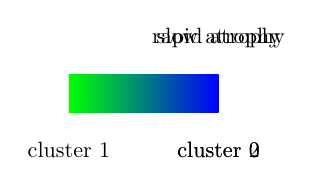
\begin{tikzpicture}[scale=1.9, every node/.style={scale=0.8}]
    \shade[left color=red,right color=green] (\gradLimLeft,2.5) rectangle (0,2.75);
    \shade[left color=green,right color=blue] (0,2.5) rectangle (\gradLimRight,2.75);
    \node[inner sep=0] (corr_text) at (\gradLimLeft,2.25) {cluster 0};
    \node[inner sep=0] (corr_text) at (0,2.25) {cluster 1};
    \node[inner sep=0] (corr_text) at (\gradLimRight,2.25) {cluster 2};
    \node[inner sep=0] (corr_text) at (\gradLimLeft,3) {rapid atrophy};
    \node[inner sep=0] (corr_text) at (\gradLimRight,3) {slow atrophy};
  \end{tikzpicture}
%     \caption{}
%       \label{fig:adniClust}
  \vspace{1em}
  \end{subfigure}
  
  %%%%%%%%%%%%%%%%%%% BRAINS %%%%%%%%%%%%%%5%%%%%%
  
  \begin{subfigure}[b]{0.3\textwidth}
   \centering
  \begin{tikzpicture}[scale=\scalingFactor, every node/.style={scale=\scalingFactor}]
    \node[inner sep=0] (image) at (0,0) {\includegraphics[width=\scalingFactorBrains\textwidth]{../images/vwdpm/blend14_adniThavgFWHM0InithistCl3Pr0Ra1_VWDPMStd.png}}; 
    \node[inner sep=0] (label) at (0,3.5) {tAD - ADNI};
  \end{tikzpicture}
%     \caption{}
%       \label{fig:adniClust}
  \end{subfigure}
   \begin{subfigure}[b]{0.3\textwidth}
  \centering
  \begin{tikzpicture}[scale=\scalingFactor]
    \node[inner sep=0] (corr_text) at (0,0) {\includegraphics[width=\scalingFactorBrains\textwidth]{../images/vwdpm/drcThavgFWHM0InithistCl3Pr0Ra1_VWDPMStdAD_blend24.png}};
    \node[inner sep=0] (label) at (0,3.5) {tAD - DRC dataset};
  \end{tikzpicture}
%     \caption{}
%       \label{fig:drcClustAD}
  \end{subfigure}
   \begin{subfigure}[b]{0.3\textwidth}
  \centering
  \begin{tikzpicture}[scale=\scalingFactor, every node/.style={scale=\scalingFactor}]
    \node[inner sep=0] (corr_text) at (0,0) {\includegraphics[width=\scalingFactorBrains\textwidth]{../images/vwdpm/drcThavgFWHM0InithistCl3Pr0Ra1_VWDPMStdPCA_blend24.png}};
    \node[inner sep=0] (label) at (0,3.5) {PCA - DRC dataset};
  \end{tikzpicture}
%     \caption{}
%       \label{fig:drcClustPCA}
  \end{subfigure}
  
  %%%%%%%%%%%%%%%%%%%%%% trajectories %%%%%%%%%%%%%%%%%%%%%%%
  
    \begin{subfigure}[b]{0.3\textwidth}
    \centering
%     \vspace{-2em}
    \includegraphics[width=\scalingFactorTraj\textwidth]{../images/vwdpm/trajSamplesOneFig_adniThavgFWHM0InithistCl3Pr0Ra1_VWDPMStd.png}
%     \caption{}
%       \label{fig:adniTraj}
  \end{subfigure}
      \begin{subfigure}[b]{0.3\textwidth}
    \centering
%     \vspace{-2em}
    \includegraphics[width=\scalingFactorTraj\textwidth]{../images/vwdpm/trajSamplesOneFig_drcThavgFWHM0InithistCl3Pr0Ra1_VWDPMStdAD.png}
%     \caption{}
%       \label{fig:drcTrajAD}
  \end{subfigure}
    \begin{subfigure}[b]{0.3\textwidth}
    \centering
%     \vspace{-2em}
    \includegraphics[width=\scalingFactorTraj\textwidth]{../images/vwdpm/trajSamplesOneFig_drcThavgFWHM0InithistCl3Pr0Ra1_VWDPMStdPCA.png}
%     \caption{}
%       \label{fig:drcTrajPCA}
  \end{subfigure}
  
%   \caption{}
%   \label{fig:clustTrajAll}

\end{figure}

\textbf{Conclusion}: We can see a fine-grained spatial distribution of atrophy.

\end{frame}

\begin{frame}
\frametitle{Future Work Plan}

\tikzset{every picture/.append style={scale=2.5}}

% Gantt chart
\begin{figure}

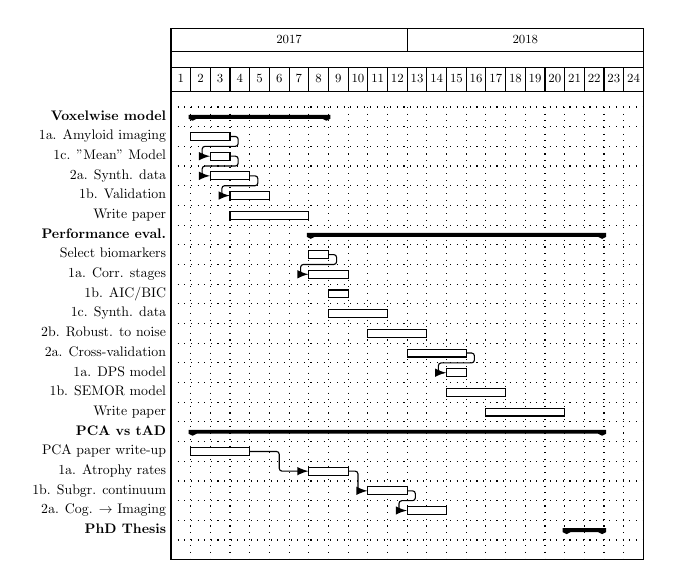
\begin{tikzpicture}[scale=0.5, every node/.style={scale=0.5}]
\begin{ganttchart}[vgrid, hgrid,y unit chart=0.5cm]{1}{24}
\gantttitle{2017}{12}
\gantttitle{2018}{12}\\
\gantttitlelist{1,...,24}{1}\\
%First Group
\ganttgroup{Voxelwise model}{2}{8} \\
\ganttbar{1a. Amyloid imaging}{2}{3} \\
\ganttbar{1c. "Mean" Model}{3}{3}\\
\ganttbar{2a. Synth. data}{3}{4}\\
\ganttbar{1b. Validation}{4}{5} \\
\ganttbar{Write paper}{4}{7}\\
%\ganttlink{elem0}{elem1}
\ganttlink{elem1}{elem2}
\ganttlink{elem2}{elem3}
\ganttlink{elem3}{elem4}
% \ganttlink{elem4}{elem5}
%\ganttmilestone{Milestone 1}{11}
%Second Group
\ganttgroup{Performance eval.}{8}{22} \\
\ganttbar{Select biomarkers}{8}{8} \\
\ganttbar{1a. Corr. stages}{8}{9} \\
\ganttbar{1b. AIC/BIC}{9}{9} \\
\ganttbar{1c. Synth. data}{9}{11}\\
\ganttbar{2b. Robust. to noise}{11}{13}\\
\ganttbar{2a. Cross-validation}{13}{15}\\
\ganttbar{1a. DPS model}{15}{15}\\
\ganttbar{1b. SEMOR model}{15}{17}\\
\ganttbar{Write paper}{17}{20}\\

\ganttlink{elem7}{elem8}
\ganttlink{elem12}{elem13}
%\ganttmilestone{Milestone 1}{11}
%Third Group
\ganttgroup{PCA vs tAD}{2}{22} \\
\ganttbar{PCA paper write-up}{2}{4}\\
\ganttbar{1a. Atrophy rates}{8}{9}\\
\ganttbar{1b. Subgr. continuum}{11}{12}\\
\ganttbar{2a. Cog. $\rightarrow$ Imaging}{13}{14}\\

\ganttlink{elem17}{elem18}
\ganttlink{elem18}{elem19}
\ganttlink{elem19}{elem20}

\ganttgroup{PhD Thesis}{21}{22} \\


\end{ganttchart}
\end{tikzpicture}
\end{figure}

\end{frame}

\begin{frame}
\frametitle{Acknowledgements}

\begin{figure}
 \begin{subfigure}{0.32\textwidth}
 \centering
 Daniel Alexander
 \includegraphics[scale=0.35]{Danny-Alexander.jpeg}  
 \end{subfigure}
  \begin{subfigure}{0.32\textwidth}
  \centering
  Sebastian Crutch
 \includegraphics[scale=0.35]{Seb_Crutch_photo.JPG}  
 \end{subfigure}
  \begin{subfigure}{0.32\textwidth}
  \centering
  Timothy Shakespeare
 \includegraphics[scale=0.2]{tim_photo.png}  
 \end{subfigure}
 \vspace{1em}
 
  \begin{subfigure}{0.25\textwidth}
 \centering
 Neil Oxtoby
 \includegraphics[scale=0.35]{neil_photo.jpg}  
 \end{subfigure}
  \begin{subfigure}{0.25\textwidth}
 \centering
 Alexandra Young
 \includegraphics[scale=0.5]{alex_photo.jpg}  
 \end{subfigure}
  \begin{subfigure}{0.3\textwidth}
  \centering
  \includegraphics[scale=0.15]{CDTlogo.png}\\
  \vspace{1em}
  \includegraphics[scale=1]{pondLogo.png}  
  \end{subfigure}

\end{figure}


\end{frame}

 
\end{document}

